\chapter{Executable Metamodelling}
\label{execChapter}

\section{Introduction}

The purpose of this chapter is to describe how the addition of
executable  primitives to a metamodelling language can result in a
powerful meta-programming environment in which many different
operational aspects of languages can be described. This includes
the ability to model the operational behaviour of a modelling or
programming language and the ability to quickly create many types
of applications to manipulate models.

\section{Why Executable Metamodelling?}

Executable metamodelling is a natural evolution of a growing trend
towards executable modelling \cite{Mellor}. Executable modelling
enables the operational behaviour of system models to be captured
in a form that is independent of how the model is implemented.
This is achieved by augmenting the modelling language with an
action language or other executable formalism. Executable models
enable a system to be tested before implementation begins,
resulting in improved validation of the system design.
Furthermore, it is also possible to generate executable code from
an executable model, as there is sufficient information to
generate method bodies, etc, in the target programming language.

The ability to execute {\em metamodels} has additional benefits
over and above those associated with executable modelling. At the
simplest level, many developers need the facility to access and
manipulate models at the metamodel level. For instance, a
developer may need to analyse general properties of their models,
or to globally modify certain features of a model, or write useful
functions that automate a time consuming modelling task. Being
able to quickly add some functionality that will perform the
required task will thus save time and improve the modelling
process.

More generally, the addition of executability to metamodels
facilitates what is almost metamodelling nirvana: the ability to
model all aspects of a modelling language as a unified, executable
entity. A static metamodel cannot model the operational behaviour
of a language. Yet, in the semantic rich tools that are required
by Language-Driven Development, capturing this aspect of a
language is essential. With an executable metamodelling language,
all of this can be described in the metamodel itself.

The advantage is that the modelling language definition becomes
completely self contained, and can be interchanged between any
modelling tool that supports the necessary metamodelling
machinery. Such definitions are not reliant on platform specific
technology but the metamodel architecture that they are defined
within (which as we shall see can itself be modelled independently
of other technologies).

\subsection{Executability and XMF}

Because XMF is also defined in terms of an executable metamodel,
XMF can effectively implement everything associated with
supporting itself as a language definition language, including the
construction of parsers, compilers, interpreters and so on. The
key advantage is that there is unification in the way that all
modelling languages are constructed. Thus, a language for
modelling StateMachines will use entirely the same meta-machinery
as a language for modelling user interactions, business use cases,
and so on. Moreover, because the definition is in effect a
program, it will be as precise and unambiguous as any program
written in a programming language. Of course, it is still
necessary that the machinery developed to support XMF is as
generic as possible to facilitate the rapid construction of new
modelling languages - being executable does not necessarily mean
that it is generic.

A unified executable metamodelling environment offers important
advantages to the language developer. We have seen many
metamodelling tools where the developer has to contend with a
multitude of ill-fitting languages for dealing with each of the
different aspects required for tool design. For instance, a
repository for dealing with meta-data, a scripting language for
model manipulation, a GUI framework for user interface design, and
lexx and yacc for parser construction. An approach in which all
these languages are unified under a single executable
metamodelling umbrella offers a far more effective and productive
development environment.

Executable metamodelling is at the heart of the tool development
vision described in chapter \ref{metamodellingChapter}. By
supporting executability, metamodels are enriched to the point
where they can support a multitude of semantically rich tool
capabilities.

\subsection{Executable Metamodelling and Programming}

How does executable metamodelling relate to programming? Not at
all? In fact it is a natural extension (see section
\ref{progvsmodel}). Rather than thinking about modelling languages
as being different to programming languages, executable
metamodelling really views modelling languages as part of a
spectrum of programming languages, where each language is only
different in the abstractions and behaviour it encapsulates.
Indeed, executable metamodelling can be thought of as next
generation programming: whilst many programming languages are
fixed in what they can represent, executable metamodelling offers
infinite extensibility and flexibility.

\section{Adding Executability}

How can executability be added to a metamodelling language? The
answer (briefly discussed in chapter \ref{xmfchapter}) is to
provide the action primitives necessary to support execution.
These in combination with a suitable model querying and navigation
language, result in a powerful metaprogramming language.

The language proposed here is XOCL (eXecutable OCL). XOCL is a
combination of executable primitives and OCL (the Object
Constraint Language). The motivations for this combination are
discussed in section \ref{differences}.

The action primitives that are provided by XOCL are as follows:

\begin{description}
\item[Slot Update] Assigns a value to a slot of an object via the
assignment expression ":=". An example of slot update might be
{\tt self.x := self.x + 1}. \item[Object Creation] Creates a new
instance of a class via a new operation on a class from which the
object is created. An example might be: {\tt fido := Dog()}.
\item[Sequential Operator] Enables two expressions to be executed
in sequence via the operator ";". For instance, {\tt
self.x:=self.x+1; self.x:=self.x+2} will result in {\tt x} being
incremented by {\tt 3}.
\end{description}

XOCL expressions can be used in the bodies of expressions
belonging to behavioural modelling elements such as operations and
mappings. The following operation is described in the context of
the class X:

\begin{lstlisting}
context X
  @Operation doIt():Integer
    self.x := self.x + 1;
    self.x
  end
\end{lstlisting}

The above primitives provide the minimal actions necessary to add
sequential executability to OCL. Concurrent execution can be
supported by adding a suitable concurrency primitive such as
fork(), which allows multiple threads of execution to be
propagated. While the majority of metamodels only require
sequential execution, there are some cases where concurrency needs
to be supported. Examples include providing models of
communication between clients and a server or in describing the
operational semantics of concurrent modelling languages.

Finally, it is important that XMF provides the necessary
architecture to support execution in an object-oriented
environment. This aspect, called a Meta-Object Protocol or MOP
will be discussed in later versions of this book.

\subsection{XOCL Extensions}

While OCL provides a number of useful imperative style constructs,
such as {\em if} and {\em for} loop expressions, there are a small
number of extensions that we have found to be very useful when
using it as a programming language. These include:
\ \\

\noindent While expressions: standard while loops as provided
by many programming languages:

\begin{lstlisting}
@While x < 10
  do x := x + 1
end
\end{lstlisting}

\noindent Find expressions: a simplified way of traversing
collections of models and finding an element that matches specific
criteria. If xset contains an x whose value is greater than zero,
y will be incremented by 1.

\begin{lstlisting}
@Find (x,set)
  when x > 10
  do
  y := y + 1
end
\end{lstlisting}

\noindent Tables provide efficient lookup over large data
structures:

\begin{lstlisting}
let table = Table() in
    table.put(key,value);
    table.get(key)
end
\end{lstlisting}

\noindent The case statement as provided by many programming
languages:

\begin{lstlisting}
@Case(x)
  x > 1 do x := x + 1;
  x = 0 do x := 2
end
\end{lstlisting}

\noindent TypeCase expressions: selects a case
statement depending on the type of object that is passed to it.

\begin{lstlisting}
@Case(x)
  Boolean do x := false;
  Integer do x := 0
end
\end{lstlisting}

\noindent Because objects are fundamental to XMF, a number of
operations are provided for accessing and manipulating their
properties:

\begin{itemize}
\item The operation of() returns the class that the object is an
instance of, e.g. StateMachines::State.of() returns XCore::Class.
\item The operation getStructuralFeatureNames() returns the names
of the slots (attribute values) belonging to an object, e.g. if x
is an instance of the class StateMachines::State, then
x.getStructuralFeatureNames() will return the set containing
"name". \item The operation get() takes a name and return the
value of the slot of that name, e.g. x.get("y") will return the
value of the slot called "y". \item The operation set() take a
name and a value, and sets the value of the slot called name to be
the value, e.g. x.set("y",10), will set the value of the slot
called "y" to 10.
\end{itemize}

\section{Examples}

The best way to understand the benefits of executable
metamodelling is to look at some real examples. This section
provides a number of examples that provide general utility
operations for manipulating metamodels. Other parts of the book
(notably chapter \ref{semanticschapter}) describe how
executability can be used to define semantics. The case study
chapters at the end the book also provide examples of executable
metamodels.

\subsection{Example 1: Model Merge}
\label{merge}

Merging the contents of two packages is a very useful capability
that has many applications, including versioning (merging
different versions of a model together) and model management
(breaking up large models into composable pieces that can be
merged into a single artefact). The following operation is defined
on a package.

\begin{lstlisting}
context Package
  @Operation merge(p:Package)
    self.contents()->collect(c1 |
      if p.contents()->exists(c2 | c1.isMergable(c2)) then
        c1.merge(c2)
      else
        c1
      end)->union(
        p.contents()->select(c2 | self.contents()->exists(c1 |
          not c1.isMergable(c2))))
  end
\end{lstlisting}

The operation merges an element belonging to the package p with an
element belonging to the contents of the package provided they are
mergeable. Note contents() is an meta-operation belonging to all
containers (see section \ref{framework}. The conditions under
which two elements are mergeable will be defined on a case by case
basis. For example, two elements may be mergeable if they have the
same name and are of the same type. If two elements are mergeable,
then the result of the merge will be defined via a merge()
operation on the elements' types.

\subsection{Example 2: Find and Replace}

This example defines a simple algorithm for finding and replacing
named elements in the contents of a Namespace. It works by
determining whether an object is a specialisation of the class
NamedElement, and then performs the appropriate substitution if
the element name matches a name in the to be replaced in the subs
list:

\begin{lstlisting}
context Namespace
  @Operation replace(subs:Set(Sub))
    @For i in self.contents
    if i.isKindOf(NamedElement) then
      if subs->exists(r | r.from = i.name) then
        i.name := subs->select(s | r.from = i.name)->sel.to
      end
    end
  end
\end{lstlisting}

\noindent Where the class Sub is defined as follows:

\begin{lstlisting}
@Class Sub
  @Attribute from : String end
  @Attribute to : String end
end
\end{lstlisting}

Applying this operation to any Namespace is now straightforward.
For instance, the operation replaceStateName() can be written like
so:

\begin{lstlisting}
context StateMachine
  @Operation replaceStateName(subs:Set(Sub))
    self.replace(subs);
    self
  end
\end{lstlisting}

This operation is a useful mechanism for performing global search
and replace on models and programs.

\subsection{Example 3: Walker}
\label{walker}

The previous example is restricted as it only applies to
Namespaces. In many situations, one wants to be able to walk over
any structure of objects in a metamodel performing arbitrary
tasks. These tasks may include find and replace, but could be
anything from constraint checking to the global invocation of
operations.

This can be achieved using a walker. A walker recursively descends
into an elements structure and dispatches to appropriate operations
depending on the values of component elements. A critical
requirements is that the walker can handle cycles in a structure.
It does this by recording the elements that have been walked, and
then using this information to ignore those elements if they are
met again.

\begin{lstlisting}
@Class Walker
  @Attribute table : Table end
  @Attribute refCount : Integer end
  @Attribute visited : Integer (?) end

  @Constructor()
    self.initWalker()
  end

  @Operation initWalker()
    self.table := Table(1000)
  end
end
\end{lstlisting}

The class Walker contains a hashkey table, in which a list of all
the walked elements is kept along with an integer reference to the
element. A count is kept of the number of elements that have been
walked along with the number of references created.

\begin{lstlisting}
context Walker
  @Operation encounter(e:Element)
    self.encounter(e,self.newRef())
  end

  @Operation encounter(e:Element,v:Element)
    // Save a reference to v against the walked value e.
    table.put(e,v)
  end

  @Operation newRef():Integer
    self.refCount := refCount + 1;
    refCount
  end
\end{lstlisting}

The encounter() operation is called when a new element is
encountered. It creates a new reference for the element, and adds
it to the table.

The following operations deal with walking the tree. The operation
encountered() returns true if the element has already been
encountered.

\begin{lstlisting}
context Walker
  @Operation encountered(e:Element):Boolean
    // Returns true when we have already walked e.
    table.hasKey(e)
  end

  @Operation getRef(e:Element):Element
    table.get(e)
  end

  @AbstractOp reWalk(e:Element,arg:Element):Element end
\end{lstlisting}


The operation walk() performs the task of walking an element. If
the element has already been encountered then the operation
reWalk() is run (this will be specialised for specific
applications, but in most cases it will do nothing). Otherwise,
depending on the type of element that is being walked, appropriate
element walkers will be called.


\begin{lstlisting}
context Walker
  @Operation walk(e:Element,arg:Element):Element
    // Walk the element e with respect to the argument.
    self.visited := visited + 1;
    if self.encountered(e)
      then self.reWalk(e,arg)
    else
      @TypeCase(e)
        Boolean      do self.walkBoolean(e,arg) end
        Integer      do self.walkInteger(e,arg) end
        Null         do self.walkNull(arg) end
        Operation    do self.walkOperation(e,arg) end
        SeqOfElement do self.walkSeq(e,arg) end
        SetOfElement do self.walkSet(e,arg) end
        String       do self.walkString(e,arg) end
        Table        do self.walkTable(e,arg) end
        Object       do self.walkObject(e,arg) end
        else self.defaultWalk(e,arg)
      end
    end
  end
\end{lstlisting}


The most complex of these walkers is the object walker. This gets
all the structural feature names of the object, i.e. the names of
the attributes of the class the object is an instance of. To do
this, it uses the {\tt getStructuralFeatureNames} operation
defined on the class Object to return the names of the structural
features. It then walks over each of the slots that correspond to
each structural feature:

\begin{lstlisting}
context Walker
  @Operation walkObject(o:Object,arg:Element):Element
    self.encounter(o);
    @For name in o.getStructuralFeatureNames() do
      self.walkSlot(o,name,arg)
    end
  end
\end{lstlisting}

Again, walkSlot() will be defined on an application basis, but in
general will simply get the element value of each slot and call its
walker.

This example illustrates the benefits of being able to program at
the meta-level. It allows the designer to produce code that is
reusable across multiple metamodels irrespective of what they
define. It does not matter whether the object that is being walked
is a StateMachine or a BusinessEntity. At the meta-level they are
all viewed as objects.

\subsection{Example 4: Meta-Patterns}

This example shows how meta-operations can stamp out a structure
over existing model elements. This can be used as the basis for
capturing libraries of reusable patterns at the meta-level.

The following operation captures a simple containership pattern,
which can be used to stamp out a containership association between
two classes and adds an add() operation to the owning class.

Given a pair of classes, c1 and c2, the operation first creates an
instance of an attribute, a, whose name is the name of c2, and
whose type is the class c2. Next, an anonymous operation is
created called c2. It takes an object x and sets the value of the
attribute name c2 to the value of x including its existing
contents. It's name is then set to "add" plus the name of c2.
Finally, both the attribute and the operation are added to the
class c1.

\begin{lstlisting}
context Root
@Operation contains(c1 : Class,c2 : Class):Element
      let a = Attribute(Symbol(c2.name),Set(c2));
          o = @Operation anonymous(x : Element):Element
                self.set(c2.name,self.get(c2.name)->including(x))
              end
      in o.setName("add" + c2.name);
         c1.add(a);
         c1.add(o)
      end
    end
\end{lstlisting}

Figures \ref{patterns1} and \ref{patterns2} show the result of
applying the operation to two classes.

\begin{figure}[htb]
\begin{center}
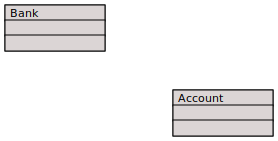
\includegraphics[width=8cm]{Programming/figures/patterns1}
\caption{An example model before applying the contains operation}
\label{patterns1}
\end{center}
\end{figure}

\begin{figure}[htb]
\begin{center}
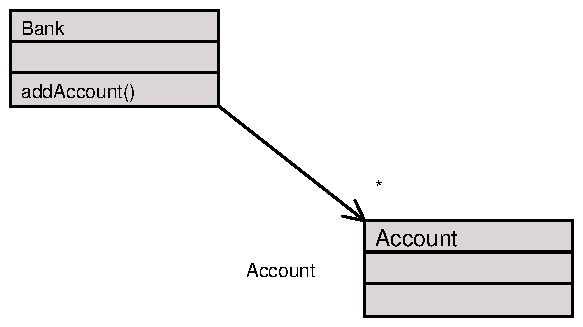
\includegraphics[width=8cm]{Programming/figures/patterns2}
\caption{An example model after applying the contains operation}
\label{patterns2}
\end{center}
\end{figure}

\section{Conclusion}

This chapter has aimed to show the benefits that can be achieved
through the extension of traditionally static metamodelling
languages to fully executable metamodelling. The resulting language
can be used in the definition of useful meta-level utility
operations right through to the construction of complete modelling
language definitions. This has wide-reaching applications for how
we treat metamodels. Rather than viewing them as static entities,
they can now be viewed as highly abstract programming devices for
language design.
